\documentclass[12pt,fleqn,answers]{exam}
\usepackage{pifont}
\usepackage{dingbat}
\usepackage{amsmath,amssymb}
\usepackage{epsfig}
\usepackage[colorlinks=true,linkcolor=black,anchorcolor=black,citecolor=black,filecolor=black,menucolor=black,runcolor=black,urlcolor=black]{hyperref}
\usepackage[letterpaper, margin=0.75in]{geometry}
\usepackage{tikz}

\usetikzlibrary{arrows}
\usepackage[super]{nth}
\usetikzlibrary{arrows}
\addpoints
\boxedpoints
\pointsinmargin
\pointname{pts}

\usepackage{pdfpages}
\usepackage[final]{microtype}
\usepackage[american]{babel}
\usepackage[T1]{fontenc}
\usepackage{fourier}
%\usepackage{eucal}

\usepackage{isomath}
\usepackage{upgreek,amsmath}
\usepackage{amssymb}
\usepackage{siunitx}

\newcommand{\dotprod}{\, {\scriptzcriptztyle
    \stackrel{\bullet}{{}}}\,}

\newcommand{\reals}{\mathbf{R}}
\newcommand{\lub}{\mathrm{lub}} 
\newcommand{\glb}{\mathrm{glb}} 
\newcommand{\complex}{\mathbf{C}}
\newcommand{\dom}{\mbox{dom}}
\newcommand{\range}{\mbox{range}}
\newcommand{\cover}{{\mathcal C}}
\newcommand{\integers}{\mathbf{Z}}
\newcommand{\degree}{\mathrm{degree}}
\newcommand{\vi}{\, \mathbf{i}}
\newcommand{\vj}{\, \mathbf{j}}
\newcommand{\vk}{\, \mathbf{k}}
\newcommand{\bi}{\, \mathbf{i}}
\newcommand{\bj}{\, \mathbf{j}}
\newcommand{\bk}{\, \mathbf{k}}
\newcommand{\dist}{\, \mathrm{dist}}
\DeclareMathOperator{\Arg}{\mathrm{Arg}}
\DeclareMathOperator{\Ln}{\mathrm{Ln}}
\newcommand{\imag}{\, \mathrm{i}}

\usepackage{tikz}
\usepackage{amsmath}
\usetikzlibrary{arrows}
\usepackage{xcolor}
\shadedsolutions
\definecolor{SolutionColor}{rgb}{0.95,0.95,0.95}

\usepackage{graphicx}
\newcommand\AM{{\sc am}}
\newcommand\PM{{\sc pm}}

\usepackage{pstricks}
\usepackage{pgfplots}
\usepackage{pst-plot}
\psset{algebraic}

%\usepackage{twemojis}
\newcommand{\quiz}{15}
\newcommand{\term}{Spring}
\newcommand{\due}{9:55 \AM}
\newcommand{\class}{MATH 102}
\begin{document}
\large
\vspace{0.1in}
\noindent\makebox[3.0truein][l]{\textbf{\class, \term \/ \the\year}}
\textbf{Name:} \hrulefill \\
\noindent \makebox[3.0truein][l]{\textbf{Final Exam Review, Part B \quiz}}
\textbf{Row and Seat}:\hrulefill\\
%\vspace{0.1in}

%\small
\begin{flushleft}
  \emph{
    “Keep cool but care.” \hfill {\sc Thomas Pynchon}, V.}
 %   “Money buys everything except love, personality, freedom, immortality, silence, peace.”}
 %   \hfill \sc{Carl Sandburg}
  %  “Sometimes it's a little better to travel than to arrive.”}  \hfill {\sc  Robert M. Pirsig}
 %   “Self-education is, I firmly believe, the only kind of education there is.” 
  %  \hfill {\sc  Isaac Asimov }}
\end{flushleft}
 \large
%\noindent  In class work  \quiz\/  has questions 1 through  \numquestions \/ with a total of  \numpoints\/  points.   
% This assignment is due at the end of the class period (\due).
%This assignment is printed on \textbf{both} sides of the paper.
%\vspace{0.1in}


\begin{questions} 

    \question Define a function $W$ by $W(x) = \sqrt{x}$ and $\dom(W) = [0,4]$. 
    Find the \emph{range} of $W$.
    \begin{solution}
      A graph of the square root function shows that $\range(W) = [0,2].$
      \end{solution}
    \question [5] Find the \emph{distance} between the points $(7,9)$ and $(-1,-2)$.
    \begin{solution}[2.0in]
    We have
    \begin{align*}
        \dist((7,9),(-1,-2)) &= \sqrt{(7+1)^2 + (9 + 2)^2}, &(\mbox{distance formula})\\
                               &= \sqrt{64+ 121}, &(\mbox{arithmetic})\\
                               &= \sqrt{185}. &(\mbox{arithmetic})
    \end{align*}
    \begin{itemize}
    
        \item It's easy to misread a question--be careful. I often put what you need to find in italic type (in this case \emph{distance})  in an attempt to clarify what you are looking for.
        
        \item The factors of 185 are $5$ and $37$.  Neither of these factors are perfect squares, so $\sqrt{185}$
        is properly simplified. 
    
        \item Unless you are asked for a decimal approximation, you should leave
        your answers in an exact form. This problem \emph{doesn't} ask for an exact 
        solution, so  $13.60147$ is \emph{not} a correct solution.
        
        \item A common error is to do the following:
        \begin{align*}
            \sqrt{8^2 + 11^2} = 8 + 11  = 19.
       \end{align*}
        But this is \textbf{wrong}. The equation $\sqrt{x^2 + y^2} = x + y$ is not an identity. You can verify this by 
        pasting in $x = 1$ and $y=1$ into the equation. The result is
         \begin{align*}
            \left[\sqrt{1^2 + 1^2} = 1+ 1 \right]  = \left[\sqrt{2} = 2 \right] = \mbox{False}
       \end{align*}
       Our Quick Reference Sheet lists other common errors.
    \end{itemize}
    
    
    
    \end{solution}
    
    \question[5] The \emph{midpoint} of points $P$ and $(5,6)$ is $(-2,3)$. Find the 
    \emph{coordinates} of the point $P$.
    \begin{solution}[2.0in] Let $P = (x,y)$. We have
        \begin{equation*}
            \left(\frac{x+5}{2}, \frac{y+6}{2} \right) = (-2,3).
        \end{equation*}
        So we need to solve
        \begin{align*}
            \frac{x+5}{2} &= -2,\\
            \frac{y+6}{2} &= 3.
        \end{align*}
        for $x$ and for $y$. Solving the first equation for $x$ gives
        \begin{align*}
            \left[  \frac{x+5}{2} = -2 \right] &= [x + 5 = -4], &\mbox{(multiply by 2)}\\
                                                &= [x=-9]. &\mbox{(add -5)}
        \end{align*}
        And solving the second for $y$ gives
        \begin{align*}
            \left[  \frac{y+6}{2} = 3 \right] &= [y+6 = 6], &\mbox{(multiply by 2)}\\
                                               &= [y=0]. &\mbox{(add -6)}
        \end{align*}
        Solving these equations for $x$ and $y$ gives $x=-9$ and $y=0$.
    
    \end{solution}
    \question A line $L$ contains the points $(x=5,y=2)$ and
    $(x=7,y=-1)$.  
    
    \begin{parts}
    
        \part [1] Find an \emph{equation} of the line $L$.
        \begin{solution}[1.5in] The slope of the line $L$ is
            \begin{equation*}
                \frac{2-(-1)}{5-7} = -\frac{3}{2}
            \end{equation*}    
            Using the point $(x=5,y=2)$ in the point-slope formula, an equation of
            the line is
            \begin{equation*}
                y-2 = -\frac{3}{2} (x-5).
            \end{equation*}
            Using the other point, gives an equation that looks different, but 
            describes exactly the same  line.
    
            \quad A good way to check our work is to paste
            the data in to the equation and see if it is true. Pasting
            $(x=5,y=2)$ into our equation for $L$, we have
            \begin{equation*}
                \left[2-2 = -\frac{3}{2} (5-5) \right] = 
                   \left[0 = 0\right] = \mbox{True}.
            \end{equation*}
            And pasting in $(x=7,y=-1)$, we have
            \begin{equation*}
                \left[-1-2 = -\frac{3}{2} (7-5) \right] = 
                   \left[-3 = -3 \right] = \mbox{True}.
            \end{equation*}
           
            The question doesn't ask for a particular form for 
            the equation of the line. We've found a point slope form for 
            the line and we have checked our work. What should we do now? We 
            should LIB (let it be).    
            If the question asked for the slope-intercept form, we would need to 
            give the answer as
            \begin{equation*}
                y = -\frac{3}{2}  x + \frac{19}{2}.
            \end{equation*} 
             But the question gives us the \emph{freedom} to give either form for
             the equation of the line.  \textbf{Let's exercise our freedom and do so.}
        \end{solution}
    
        \part  [1] Find the \emph{x-intercept} of the line $L$.
        \begin{solution}[1.5in] To find the x-intercept of the line
            $y-2 = -\frac{3}{2} (x-5)$, set $y$ to zero and solve for $x$; we have
            \begin{align*}
                \left[0-2 = -\frac{3}{2} (x-5) \right] &= 
                    \left[\frac{4}{3}  = x-5 \right],  &\mbox{(multiply by $-2/3$)}\\
                           &= \left[x = \frac{19}{3} \right]. &\mbox{(add 5)}
            \end{align*}
    
    
        \end{solution}
    \end{parts}

    \question [5] The number of lawns $L$ a work crew can mow in a day 
varies jointly with the number of people $N$ in the crew and with
the time $T$  they work in a day.

Given that $L = 8$ when $N = 5$ and $T = 6$, find $L$ when
$N = 8$ and $T = 10$.
\begin{solution}[3.5in]
There is a constant $k$ such that $L =k N T$. This formula should make sense--doubling the size of the work crew, we
should be able to mow twice as many lawns--the formula shows that is true. The same is true for working twice as long.

Pasting in $L = 8$ when $N = 5$ and $T = 6$ into $L =k N T$ yields $8 = 30 k$.  So $k = \frac{4}{15}$.  That makes
our formula
\begin{equation*}
L = \frac{4}{15} N T.
\end{equation*}
Pasting in $N = 8$ and $T = 10$ gives
\begin{equation*}
L = \frac{4}{15} \times 80 = \frac{64}{3} \approx 21.3.
\end{equation*}


\textbf{Teacher's embellishment} A century or so ago, students were taught 
a short-cut method for such problems called the \emph{double rule of three}.
The Lewis Carroll poem ``The Mad Gardener's Song'' refers to this method.


\end{solution}

\question Find the \emph{vertex} of each parabola

  \begin{parts}

    \part[2] $y - 8 = x^2$

    \begin{solution}[1.5in] Matching $y - 8 = x^2$ to $y - k = a (x-h)^2$
      gives $k=8, h=0$, and $a=1$.  So the vertex is the point $(0,8)$.

    \end{solution}

    \part[2] $y - 8 = \sqrt{2} (x + 2)^2$

    \begin{solution}[1.5in] Matching $y - 8 = \sqrt{2} (x + 2)^2$ to $y - k = a (x-h)^2$
      gives $k=8, h=-2$, and $a=\sqrt{2}$.  
      So the vertex is the point $(-2,8)$.


    \end{solution}

        \part[2] $y=2 {{x}^{2}}-28 x+103$

   
    \begin{solution}[1.5in] Matching $y=2 {{x}^{2}}-28 x+103$ to
      $y=a x^2 + b x + c$ gives $a=2,b=-28$, and $c=103$. The 
      vertex  is the point
      \begin{equation}
        \left(-\frac{b}{2 a}, c - \frac{b^2}{4 a}\right) = 
        \left(-\frac{-28}{2 \times 2}, 103 - \frac{(-28)^2}{4 \times 2}\right) = 
        \left(7, 5 \right).
      \end{equation}
    \end{solution}

    \part[2] $y=3 (x-2)(x-4)$
    \begin{solution} To match $y=3 (x-2)(x-4)$ to $y=a x^2 + b x + c$,
      we need to expand (use FOIL) $y=3 (x-2)(x-4)$. We have
      \begin{equation*}
          y = 3 (x-2)(x-4) = 3(x^2 -6 x + 8) = 3 x^2 - 18 x + 24.
      \end{equation*}
      So $a=3, b=-18$, and $c=24$. The 
      vertex  is the point
      \begin{equation*}
        \left(-\frac{b}{2 a}, c - \frac{b^2}{4 a}\right) = 
        \left(-\frac{-18}{2 \times 3}, 24 -\frac{(-18)^2}{4 \times 3} \right) =
        \left( 3, -3 \right).
      \end{equation*}
    \end{solution}


  \end{parts}

  \question Follow these steps to solve the inequality $x^2 - x \geq 12$.

  \begin{parts}

    \part [2] \emph{Solve} the equation $x^2 -x = 12$.

    \begin{solution}[2.0in]
      \begin{align*}
        \left[x^2 -x = 12 \right] &= \left[x^2 -x -12 =0 \right]  &\mbox{(subtract 12)}\\
                    &= \left[(x-4)(x+3) =0 \right]  &\mbox{(factor)}\\
                    &= \left[x=4 \mbox{ or } x=-3  \right] & \mbox{(teacher's pet fact)}      
      \end{align*}

    \end{solution}

    \part [2] Check that \emph{both of your solutions are correct} by 
    pasting them into the equation $x^2 -x = 12$.

    \begin{solution}[2.0in]
      Pasting in $x \to 4$ into $x^2 -x = 12$ gives
      \begin{equation*}
          \left[4^2 - 4 = 12\right] = [12=12] = \mbox{True!}
      \end{equation*}
      And Pasting in $x \to -3$ into $x^2 -x = 12$ gives
      \begin{equation*}
          \left[(-3)^2 + 3 = 12\right] = [12=12] = \mbox{True!}
      \end{equation*}

    \end{solution}

    \part [2] Put both of your solutions on a \emph{number line}, correctly
    ordered from \emph{least to greatest}.

    \begin{solution}%[1.0in]

      \usetikzlibrary{arrows}
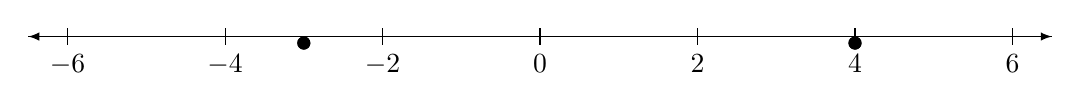
\begin{tikzpicture}
\draw[latex-] (-6.5,0) -- (6.5,0) ;
\draw[-latex] (-6.5,0) -- (6.5,0) ;
\foreach \x in  {-6,-4,-2,0,2,4,6}
\draw[shift={(\x,0)},color=black] (0pt,3pt) -- (0pt,-3pt);
\foreach \x in {-6,-4,-2,0,2,4,6}
\draw[shift={(\x,0)},color=black] (0pt,0pt) -- (0pt,-3pt) node[below] 
{$\x$};
%\draw[*-o] (-3,-3) -- (-3,-3)
\draw[*-o] (-3,0);
\draw[*-o] (4,0);
\end{tikzpicture}

    \end{solution}

  %  \vfill
  %  \newpage

    \part [2] Make a \emph{table} of the intervals determined by the number line 
    from the previous part, the test points, and the
    value of $x^2 - x \geq 12$ at each test point.
        
    \begin{solution}[4.0in]

      \begin{tabular}{|c|c|c|c|} \hline \hline 
        \textbf{Interval} &  $\mathbf{x}$  & $\mathbf{x^2 -x \geq 12}$  & \textbf{true or false}\\ \hline 
        $(-\infty,-3)$  & -4 &  $(-4)^2 + 4 \geq 12 $ & true \\  \hline 
        $(-3,4)$  & 0 &  $0^2 + 0 \geq  12 $  &false \\ \hline 
        $(4, \infty)$  & 5 &  $5^2 + 4 \geq 12 $ & true  \\ \hline        
      \end{tabular}

    \end{solution}


    \part [2] Finish the sentence:  The solution set is

    \begin{solution}
    $(-\infty, -3] \cup [4 ,\infty)$. 
    
    We include the endpoints in each interval (use a bracket, not a paren) because we're
    solving $x^2 - x \geq 12$. And that allows equality. Here in 
    a bit, this rule will be modified.

    \end{solution}

  \end{parts}

  \question Find the solution set to $\frac{2 x + 3}{4 x +1} \leq 1$ by
following these steps.

\begin{parts}

    \part [1] Use algebra tools to find an equivalent inequality of the 
    form $\frac{P(x)}{Q(x)} \leq 0$, where $P$ and $Q$ are polynomials.

    \begin{solution}[1.25in] We have
        \begin{align*}
            \left[\frac{2 x + 3}{4 x +1} \leq 1 \right] &=
               \left[\frac{2 x + 3}{4 x +1} -1 \leq 0\right], & \mbox{(subtract 1)}\\
               & = \left[\frac{2 x + 3}{4 x +1} - \frac{4 x + 1}{4 x +1} \leq 0\right], & \mbox{(make a common denominator)}\\
               &= \left[\frac{-2 x + 2}{4 x +1} \leq 0\right]. & \mbox{(combine numerators)}
        \end{align*}
    
    \end{solution}

    \part[1] Find all x-intercepts and all VAs for $\frac{P(x)}{Q(x)}$.

    \begin{solution}[2.25in] To find the x-intercepts we set the numerator to zero and solve:
        \begin{equation*}
             \left[-2x + 2 = 0\right] = \left[x=1\right].
        \end{equation*}
        To find the VA we set the denominator to zero and solve:
        \begin{equation}
             \left[4x+1 = 0\right] = \left[x= -\frac{1}{4}\right].
        \end{equation}
    
    \end{solution}


    \part [1] Put all x-intercepts and VAs on to a number line.

    \begin{solution}%[1.25in]
        \usetikzlibrary{arrows}
        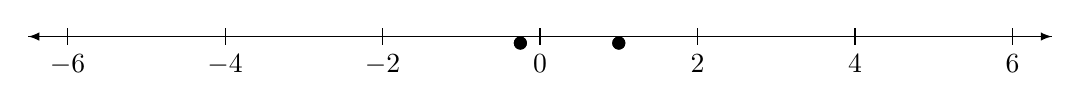
\begin{tikzpicture}
        \draw[latex-] (-6.5,0) -- (6.5,0) ;
        \draw[-latex] (-6.5,0) -- (6.5,0) ;
        \foreach \x in  {-6,-4,-2,0,2,4,6}
        \draw[shift={(\x,0)},color=black] (0pt,3pt) -- (0pt,-3pt);
        \foreach \x in {-6,-4,-2,0,2,4,6}
        \draw[shift={(\x,0)},color=black] (0pt,0pt) -- (0pt,-3pt) node[below] 
        {$\x$};
        \draw[*-o] (-0.25,0);
        \draw[*-o] (1.0,0);
       % \draw[*-o] (0.92,0) -- (2.08,0);
       % \draw[very thick    ] (0.92,0) -- (1.92,0);
        
        \end{tikzpicture}
    \end{solution}

    \vfill 
    \newpage
    \part [1] Build the chart with columns for the interval, the test
    number, evaluation at the test number, and the true/false value.

    \begin{solution}[3.25in]
    
    \begin{tabular}{|c|c|c|c|}
    \hline
     \textbf{Interval} & \textbf{Test} & $\frac{2 x + 3}{4 x +1} \leq 1$ & \textbf{True or False} \\ \hline
     $(-\infty, -1/4)$  & -1  & $-\frac{1}{3} \leq 1$ & True \\
      $(-1/4,1)$  &  0  & $3 \leq 1 $ & False \\
      $(1,\infty)$ & 2 & $\frac{7}{9} \leq 1$ & True \\ \hline
    \end{tabular}
    
    \end{solution}


    \part [1] Test each interval endpoint for inclusion or
    exclusion into the solution set.

    \begin{solution}[3.25in]
    
 \begin{tabular}{|c|c|c|}
 \hline
   \textbf{Endpoint} &  $\frac{2 x + 3}{4 x +1} \leq 1$ & \textbf{True or False} \\ \hline
    $-1/4$   & dne   & False \\
    1           & $1 \leq 1$ & True \\ \hline
 \end{tabular}
    
    \end{solution}

    \part [1] Express the solution set in either interval notation, 
    pictorially, or set builder notation.
    
    \begin{solution}
    In interval notation the solution set is $(-\infty,-\frac{1}{4}) \cup [1,\infty)$. In set builder notation,
    it is $\{x |  x < -\frac{1}{4} \mbox{ or }  x \geq  1 \}$.
    
    \end{solution}

\end{parts}

\question [2]  At 6 \AM,\, Louisa has 340 mg of caffeine circulating 
in her blood. After $T$ hours, the amount of caffeine $C$ in her blood is
\(
     C = 340  \times  0.9^T
\).
When Louisa goes to bed at 10 \PM,\, how much caffeine is
still in circulation?
\begin{solution}[1.5in] We have
    \begin{equation*}
        C = 340 \times 0.9^{16} = \SI{63.0}{\milli\gram}.
    \end{equation*}
I rounded the value to the nearest tenth---given the context, that
is reasonable.
\end{solution}


\question Find the inverse of the function $f(x) = \frac{2 x + 1}{x-1}, \,\, x \neq 1$.
\begin{solution}[2.5in]
    We need to solve $y = \frac{2 x + 1}{x-1}$ for $x$. 
    When $y = 2$, the solution set is empty; otherwise, the
    solution is 
    \begin{equation*}
         x = \frac{y+1}{y-2}                           
    \end{equation*}
    So $f^{-1}(y) = \frac{y+1}{y-2}$ and $\dom(f^{-1}) = \{y | y \neq 2 \}$.
        
 
\end{solution}
\end{questions}
%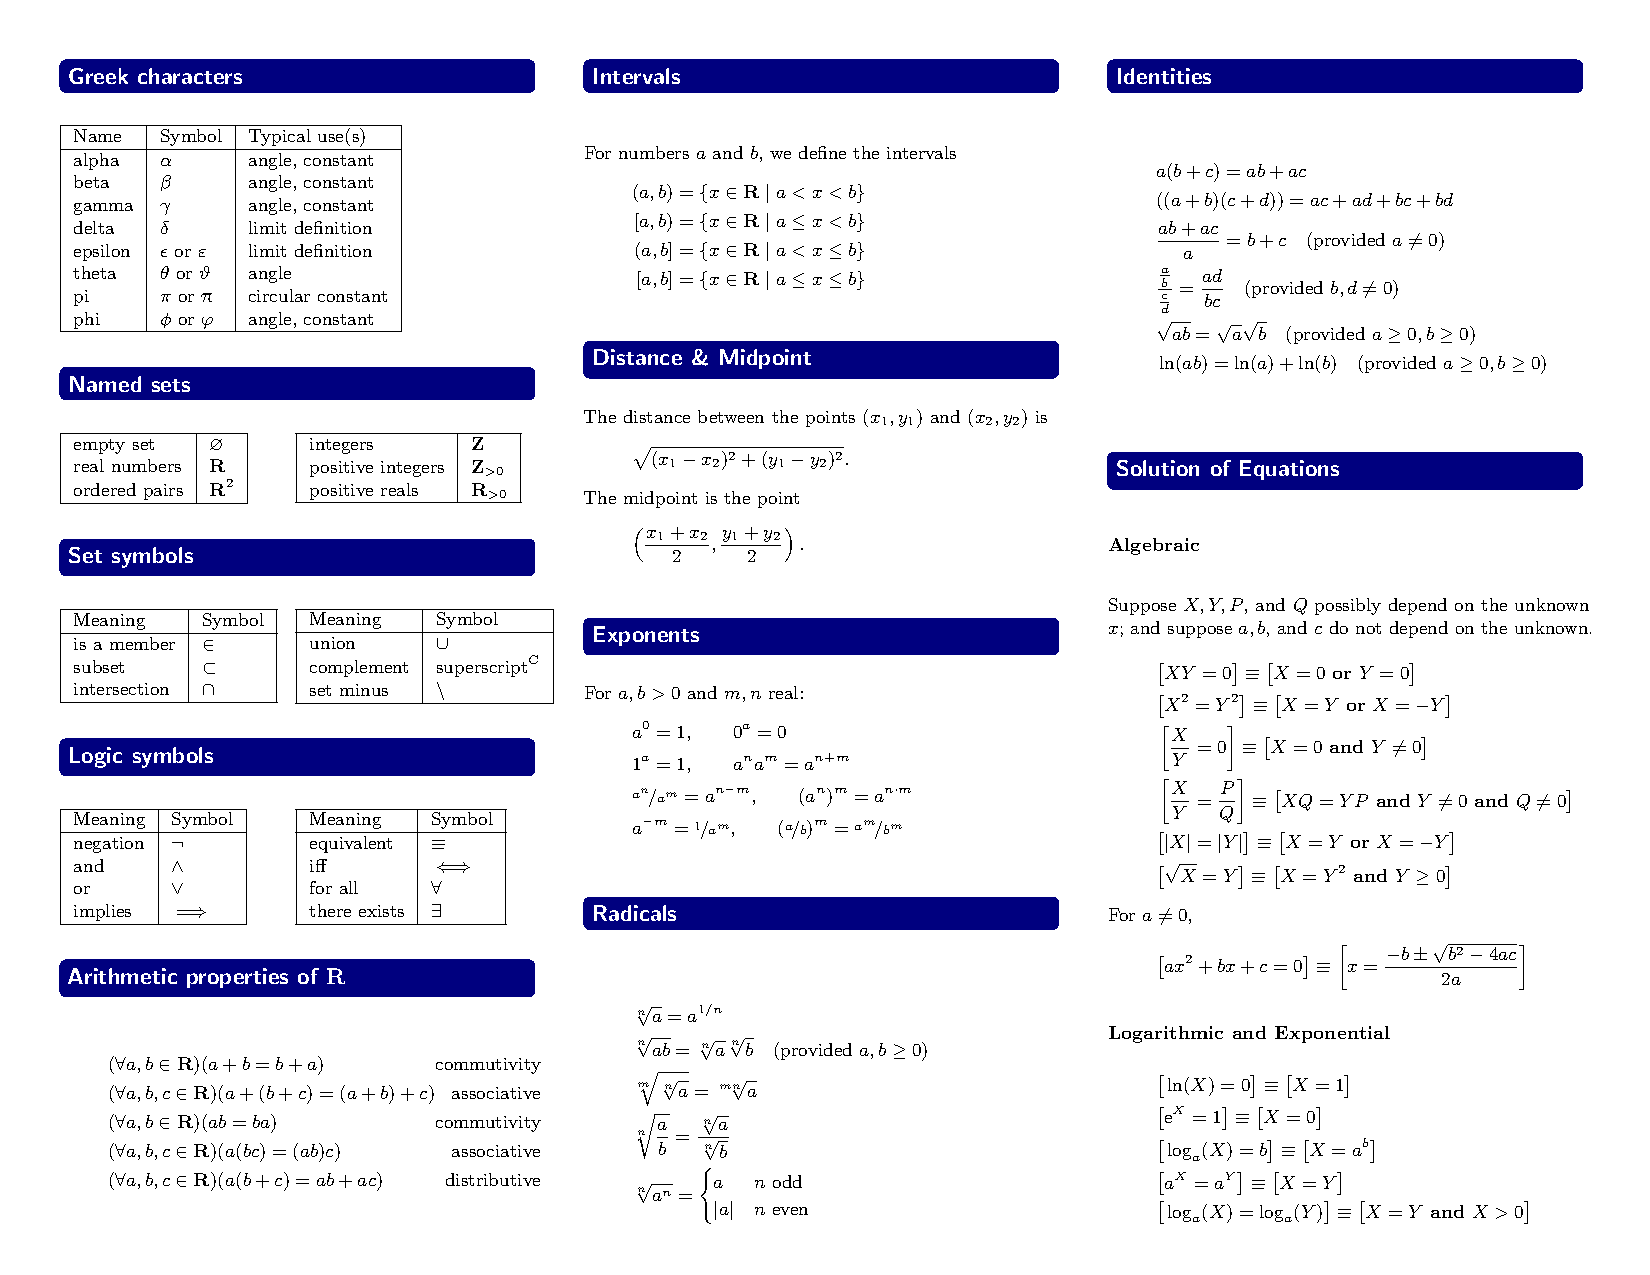
\includepdf[pages=-]{college-algebra-quick-reference}
\end{document}
